\documentclass[twoside,a4paper]{article}

\usepackage{graphicx}
\usepackage{url}
\usepackage{listings}
\usepackage{color}

\definecolor{dkgreen}{rgb}{0,0.6,0}
\definecolor{gray}{rgb}{0.5,0.5,0.5}
\definecolor{mauve}{rgb}{0.58,0,0.82}

\lstdefinelanguage{Thicket}
{  
  morekeywords={
    adapter, module,from, import, export,
    type, enum, trait, model, class, 
    def, let, in, if, for, yield, 
    new, with
  },
  alsoother={-><?()},
  sensitive=true, % keywords are not case-sensitive
  morecomment=[l]{//}, % l is for line comment
  morecomment=[s]{/*}{*/}, % s is for start and end delimiter
  morestring=[b]" % defines that strings are enclosed in double quotes
}

\lstset{
  numbers=left,
  stepnumber=1,
  aboveskip=3mm,
  belowskip=3mm,
  showstringspaces=false,
  columns=flexible,
  basicstyle={\ttfamily},
  numberstyle=\tiny\color{gray},
  keywordstyle=\color{blue},
  commentstyle=\color{dkgreen},
  stringstyle=\color{mauve},
  breaklines=true,
  breakatwhitespace=false,
  tabsize=4
}

\lstset{language=Html}

\lstset{
 morekeywords={ adapter, module,from, import, export,
    typedef, type, trait, model, class, 
    def, let, in, if, for, yield, 
    new, with}
}

\lstset{
literate={~} {$\sim$}{1}
}

\usepackage[utf8]{inputenc}
% \usepackage[latin1]{inputenc}
\usepackage[T1]{fontenc}
\usepackage{actes}
\usepackage[french]{babel}
\title{ Du Web fonctionnel avec le langage Thicket }
\author{Didier Plaindoux$^1$}
% les titres de haut de pages
\titlehead{ Du Web fonctionnel avec le langage Thicket }%  a droite (page impaire)
\authorhead{Didier Plaindoux}% a gauche (page paire)
\affiliation{\begin{tabular}{rr} 
    \\ 1:  Fungus, Le village 31430 Gratens, France
    \\     {\tt d.plaindoux@fungus.fr}
\end{tabular}}

\begin{document}

\setcounter{page}{1}
\maketitle

\begin{abstract}
Nous pouvons  constater actuellement,  dans le monde  du développement
logiciel,   une  forte   adoption   du   paradigme  fonctionnel.   Les
applications  dites   Web  comptent  parmi  les   vecteurs  les  plus
importants pour la promotion de  cette approche. Ceci est notamment le
fait de langages fonctionnels fortement typés tels que Eml, Purescript
ou ScalaJS pour  ne citer qu’eux. Cependant ces  derniers reposent sur
un schéma  de compilation  procédant par  une “transpilation”  vers le
langage cible Javascript.

Cet article  court propose  d'aborder le  développement d'applications
clientes Web avec le langage  Thicket. Ce langage s’inscrit dans cette
mouvance des langages fonctionnels fortement  typés qui ciblent le Web
tout  en  y  intégrant  une  machine  virtuelle  spécifique  pour  son
exécution. Il dispose  de plus de constructions  syntaxiques dédiées à
la  dénotation  de  termes  HTML   afin  de  proposer  une  expression
déclarative de  la composition  de documents. Nous  verrons finalement
comment  ce langage  peut être  intégré  dans un  client. Cela  couvre
notamment le schéma  de compilation traditionnel mais  aussi un schéma
de compilation dit à la volée.
\end{abstract}

\section{Introduction}

Des   langages   tels  que   OCaml   \cite{ocaml}   ou  bien   Haskell
\cite{haskell}   ont   permis   d'étendre   l'adoption   de   langages
fonctionnels. Cependant, ces dernières  années ont vu une accélération
de cette adoption  via des langages hybrides  comme Scala \cite{scala}
ou bien Java \cite{java} et son extension aux lambdas.

En parallèle,  cet engouement  se trouve  aussi porté  par le  Web qui
accentue cette  mouvance. Ceci  est le  fait de  langages fonctionnels
fortement typés tels que  Eml \cite{elm}, Purescript \cite{purescript}
ou ScalaJS \cite{scalajs} pour ne citer qu’eux.

Ces dernières  approches soulèvent cependant deux  problématiques.  La
première  concerne l'expressivité  du langage  et notamment  lorsqu'il
s'agit de manipuler le DOM \cite{dom}.   En effet, à l'instar de React
\cite{react} ou Angular  \cite{angularjs} qui sont centrés  sur le DOM
et sa  manipulation, la plupart  des solutions proposent  une approche
fonctionnelle de la  construction des balises HTML rendant  de ce fait
difficile la  conception.  La  seconde concerne le  modèle d'exécution
qui nécessite la  plupart du temps une  transpilation vers Javascript.
Malgré les étapes  d’optimisation mises en oeuvre  comme le traitement
spécifique  de la  récursion  terminale, une  telle transformation  ne
permet pas d’avoir une maîtrise totale  du langage et de son exécution
comme  cela peut  être  le  cas avec  le  support  d’une machine  SECD
spécifique.

Lors  de  l'élaboration du  langage  Thicket  \cite{thicket} ces  deux
problématiques  ont   été  particulièrement  ciblées   afin  d'étudier
l'expressivité et  l'intégration dans le monde  des applications dites
Web.  Dans un premier temps  nous faisons une présentation très rapide
du  langage.    Cela  couvre  l'expressivité  et   notamment  l'aspect
déclaratif pour les éléments visuels.  L'intégration dans un processus
d'élaboration d'application Web sera finalement abordée.

\section{Survol (très rapide) du langage}

Thicket  est  un  langage  fonctionnel  fortement  typé  à  évaluation
paresseuse non-stricte  intégrant le paradigme objet  par l'apport des
traits \cite{trait}  et reposant sur  un principe de  séparation entre
les classes et les modèles quelles dénotent.

Nous  proposons  un survol  très  rapide  du  langage en  couvrant  la
représentation des données et  leurs manipulations. Un point important
concerne l'absence d'effet de bord  conférant au langage une propriété
dite d'immutabilité.   Ce dernier point est  important notamment quand
sera abordé le cycle de vie d'une application dite Web.

\subsection{Modèle de données}

Une  donnée est  dénotée par  une expression  de type  enregistrement.
Ainsi,  toute  donnée  secondaire  est alors  accessible  par  le  nom
associé.   Une   données  est   ainsi  représentée  par   un  ensemble
d'attributs typés comme suit:

\lstset{language=Thicket}
\begin{lstlisting}
  model Personne {  
    nom: string   
    age: number
  }
\end{lstlisting}

Un  générateur pour  le type  {\tt Personne}  est alors  naturellement
synthétisé  avec une  signature calquant  le type  des attributs  dans
l'ordre  de  spécification.   Construire   une  donnée  de  type  {\tt
  Personne} correspond  alors à  appliquer cette fonction.   Une telle
définition n'est  pas sans  rappeler la définition  de type  de donnée
avec enregistrements en Haskell \cite{haskell}.

\lstset{language=Thicket}
\begin{lstlisting}
  Personne "Anakin Skywalker" 1 
\end{lstlisting}

De  cette donnée  il  est  alors aisé  d'extraire  une information  en
procédant    par   le    nommage    spécifique    de   la    propriété
souhaitée \footnote{Au même  titre que Scala la formulation  {\tt o m}
  est équivalent à {\tt o.m} dans  le cadre de la selection d'attribut
  des modèle et de méthode de classe.}.

\lstset{language=Thicket}
\begin{lstlisting}
  Personne "Anakin Skywalker" 1 nom
\end{lstlisting}

Le  langage propose  aussi  la définition  de  données pouvants  avoir
plusieurs formes  par leurs énumérations  au même titre que  les types
injectifs  \cite{ocaml}   \cite{haskell}  ou  les  {\it   case  class}
\cite{scala}.  Par  contre, le filtrage  de formes simples  repose sur
l'application     de    catamorphismes     \cite{meijer1991functional}
spécifiques.

\subsection{Manipulation des données}

Une classe  est un générateur  prenant en paramètre une  expression et
proposant en retour une base de connaissances.

\lstset{language=Thicket}
\begin{lstlisting}
  class jedi personne:Personne {
    nom: string
    grade: string
  } {
    def nom = personne.nom
    def grade = personne.age <? 21 fold "Padawan" "Maitre"
  }
\end{lstlisting}

La création  d'une instance  de classe consiste  alors à  appliquer le
générateur associé à une donnée de type {\tt Personne}.

\lstset{language=Thicket}
\begin{lstlisting}
  jedi (Personne "Anakin Skywalker" 1)
\end{lstlisting}

Finalement, l'activation d'une méthode consiste en un envoi de message
à l'instance.

\lstset{language=Thicket}
\begin{lstlisting}
  jedi (Personne "Anakin Skywalker" 1) grade
\end{lstlisting}

Cette  approche permet  de séparer  le  modèle du  contrôleur ou  plus
généralement le signifiant du signifié.  Ce principe induit un système
avec lequel plusieurs niveaux  d'interprétation d'une même donnée peut
être simplement élaboré.

\subsection{Immutabilité et système évolutif}

Un  des principes  de base  adopté  lors de  l'élaboration du  langage
concerne  l'immutabilité. Pour  ce faire  toute donnée  est considérée
comme constante et ne peut donc être alors modifiée. L'unique approche
possible en terme de manipulation  consiste à proposer un système basé
sur l'évolution de données via un jeu de fonctions dites anamorphiques
\cite{meijer1991functional}.  Cette  approche peut  être naturellement
exprimée dans les  langages fonctionnels comme Haskell  ou OCaml privé
du {\tt mutable}.  Dans des  langages récents comme Swift \cite{swift}
il est  aussi proposé une notion  de structure pour laquelle  un objet
peut  évoluer par  copie partielle  impliquant ainsi  cette notion  de
changement sans modification de l'objet de départ.

Dans Thicket afin de faciliter l'expression d'une telle transformation
il est  possible de produire  une nouvelle  version de données  par le
biais d'une structure  de contrôle spécifique comme  cela est illustré
dans le code suivant.

\lstset{language=Thicket}
\begin{lstlisting}
  new Personne "Anakin Skywalker" 19 with nom = "Darth Vader"
\end{lstlisting}

Cette   même  structure   de  contrôle   permet  aussi   d'opérer  sur
l'expression dénotée  par une  instance de classe  et permet  ainsi de
faire évoluer le comportement associé à une base de connaissance d'une
instance dans le temps.

\lstset{language=Thicket}
\begin{lstlisting}
  class jedi personne:Personne {
    nom: string
    grade: string
    anniversaire:  jedi
  } {
    def nom = personne nom
    def grade = personne age <? 21 fold "Padawan" "Maitre"
    def anniversaire = jedi new personne with age = (personne age + 1)
  }
\end{lstlisting}

Par ce survol rapide nous avons exposé les principes de bases qui nous
ont conduit à la définition et  à l'élaboration du langage Thicket.  A
noter qu'il repose sur  des concepts parfaitement maîtrisés concernant
le typage mais aussi l'aspect fonctionnel.

\subsection{Cas de la manipulation du DOM}

Le point qui va nous intéresser maintenant concerne l'intégration d'un
tel langage dans  le monde des applications dites  Web.  Cela concerne
la  représentation  des  données  pour  le support  HTML  via  le  DOM
\cite{dom}. En effet, dans la majorité  des solutions la mise en forme
et la création de documents sont  prisent en charge par des librairies
fonctionnelles manipulant des termes du DOM \cite{dom}.

Il existe  cependant une approche  déclarative - par opposition  à une
approche constructive -  permettant d'exprimer des fragments  et ce, de
manière plus intuitive comme cela  est notamment le cas dans AngularJS
\cite{angularjs} et React \cite{react}.

\subsubsection{Expression de la structure d'un fragment}

Notre  approche repose  sur  une approche  déclarative  qui est  alors
transformée  en   expression  fonctionnelle   lors  de  la   phase  de
compilation.   Une telle  approche  permet de  combiner  une vue  plus
intuitive de la  construction de modèle de document  sans corrompre le
système de typage.

\lstset{language=Thicket}
\begin{lstlisting}
  def vueJedi : jedi -> dom = j -> <p  id="jedi"> j.grade " " j.nom </p> 
\end{lstlisting}

Bien évidemment au même titre que des langages fonctionnels1 comme Elm
et  Purescript   cette  aspect  déclaratif  peut   être  remplacé  par
l'utilisation des librairies dédiées de la façon suivante:

\begin{lstlisting}
  def vueJedi : jedi -> dom = j -> {
      document "p" create 
                     addAttribute "id" "jedi" 
                     addChild j.grade addChild " " addChild j.nom
  }
\end{lstlisting}

Cette  approche fonctionnel  permet de  créer un  élément du  DOM sans
qu'il soit  nécessairement rattaché au document  courant.  Cela permet
ainsi  de construire  virtuellement  l'ensemble  des vues  nécessaires
avant des les appliquer.

\subsubsection{Manipulation et système réactif}

Un deuxième  aspect de la  manipulation de DOM  concerne l'intéraction
avec l'extérieur.   Dans notre approche  le comportement associé  à un
noeud du DOM est séparé de  sa représentation.  Il devient alors ainsi
aisé de concevoir des systèmes réactifs par la mise en place de points
d'appels permettant de ce fait  d'appréhender la structure du document
et des comportements associées.

\begin{lstlisting}
  def vueJedi : jedi -> dom = j -> {
    <p id="jedi"> j.grade " "  j.nom </p> 
    onMouseEvent MouseClick $ n -> console log "Click ..."
  }
\end{lstlisting}

La combinaison  de cette forme  réactive avec l'approche  évolutive va
nous  permettre  de  modéliser  simplement  les  applications  Web  en
proposant     une     approche    architecturale     unidirectionnelle
\cite{unidirectionnal} en  y intégrant  la réception et  le traitement
des intéractions en  terme de changement de données  qui sera finalisé
par la phase rendue.
 
Dans notre exemple,  ceci peut être simplement mis en  évidence par la
combinaison  d'un  élément  visuel,  d'un capteur  d'évènement  et  la 
fonction de traitement associée.

\begin{lstlisting}
  def vueJedi : jedi -> dom = j -> {
    <p id="jedi"> j.grade " "  j.nom </p> 
    onMouseEvent MouseClick $ _ -> documentRenderer <~ $ vueJedi j.anniversaire
  }
\end{lstlisting}

L'élément clé dans l'exemple précédent  concerne la phase de rendu qui
permet  par appel  récursif  de  lier un  contexte  d'exécution et  la
représentation  visuelle  associée.   Ainsi à  chaque  intéraction  un
nouvel élément  visuel est produit pour  un {\tt jedi} ayant  fêter un
nouvel anniversaire.

\section{Une intégration Web sur mesure}

Afin de  proposer une  intégration dans  le monde  du Web,  la version
initiale du  compilateur a été  écrite en Javascript.   Cette approche
nous  permet dès  le départ  d'avoir une  prise en  charge du  langage
quasi-naturelle.   Conjointement  à  ce choix  le  modèle  d'exécution
proposé ne  repose pas sur une  traduction du langage vers  le langage
cible   à   savoir   Javascript   pour  le   moment   et   WebAssembly
\cite{rossberg2016webassembly} plus tard probablement.

Concernant le  langage Thicket,  le choix est  bien au  contraire plus
classique car le code  va dans un premier temps -  après les phases de
validations -  être transformé en code  objet. Ce même code  objet est
alors pris en  charge par une machine  de Krivine \cite{krivine:2007}.
Le  choix d'un  langage paresseux  non-strict nous  a dirigé  vers une
solution  plus spécifique  qui s'inspire  du jeu  d'instruction de  la
"Zinc  Abstract   Machine"  \cite{zinc}   étendue  aux  objets   et  à
l'évaluation par nécessité.

Cette approche offre - comparativement à la transpilation - l'avantage
de  découpler   l'exécution  du   code  de  l'infrastructure   qui  la
porte. Cele  permet ainsi d'avoir une  main mise totale sur  le modèle
d'exécution et de l'outillage associé.

\subsection{Analyse, compilation à la volée et exécution}

En  terme  d'élaboration  d'application,  le  code  source  peut  être
directement   embarqué   au   même   titre  qu'un   code   source   en
Javascript. Une  telle approche permet  d'avoir le même  apport qu'une
boucle d'évaluation  à savoir offrir un  prototypage rapide. Cependant
la contre-partie est  une compilation à la volée et  donc une phase de
validation pouvant lever des erreurs dans le client.

\lstset{language=Html}
\begin{lstlisting}
  <html lang="en">
  <head>
    <script type="application/thicket+package" data-src="Jedi"></script>
    <script type="application/thicket">
      from Jedi import vueJedi, jedi, Personne
      documentRenderer <~ $ vueJedi $ jedi $ Personne "Obi-Wan Kenobi" 1
    </script>

    <script src="/thicket/build/thicket-web-lang.min.js"></script>    
    <script type="application/javascript">
      function onLoad() { require('thicket')('/site').boot(); }
    </script>
  </head>        
    <body onload="onLoad()"> <div id="jedi"/> </body>
  </html>
\end{lstlisting}

Une application Web  consiste alors dans un premier  temps à spécifier
le  paquetage utilisé  (ligne 3)  ainsi  que le  programme à  exécuter
(lignes 5  et 6).   Pour la prise  en charge du  langage (ligne  9) le
compilateur   et  l'exécuteur   sont  chargés   et  finalement   quand
l'application est prête, l'analyse peut être enclenchée (ligne 11).

\begin{figure}[h]
\centering
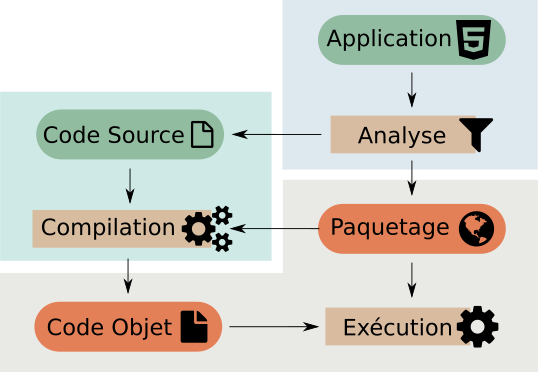
\includegraphics[scale=0.45]{repl} 
\caption{Schémas de compilation et exécution}
\label{repl}
\end{figure}

L'exécution repose sur  trois phases. La première  consiste à analyser
le DOM pour la détection des paquetages à charger et les blocs de code
source à compiler et exécuter. La seconde étape consiste à compiler et
charger  les  codes  objets  générés.  Finalement  la  dernière  étape
consiste à exécuter chacun des codes binaires à savoir les expressions
au plus haut niveau i.e. ligne 6 de notre exemple.

La figure \ref{repl}  met en évidence une compilation dite  à la volée
mais  aussi  trois étapes  clairement  identifiées  avec un  périmètre
délimité permettant de mettre en oeuvre  de bout en bout l'analyse, la
compilation et l'exécution du code.

Un point qui n'est pas abordé  ici concerne la notion de paquetage qui
est une unité de distribution contenant l'ensemble des spécifications,
le  code  objet associé  ainsi  que  l'ensemble des  dépendances  avec
d'autres paquetages.   Tout code natif javascript  référencé est aussi
embarqué permettant de définir une unité de distribution consistante.

\subsection{Analyse et exécution}

La modularisation mise en évidence  dans la figure \ref{repl} ouvre de
nouvelles perspectives comme  par exemple l'usage de  la compilation à
priori  comme  cela est  traditionnellement  mis  en oeuvre  pour  les
langages compilés.

Ainsi  la  phase d'analyse  peut  être  revisitée  afin de  mettre  en
évidence l'ensemble des code objets à exécuter.

\lstset{language=Html}
\begin{lstlisting}
  <html lang="en">
  <head>
    <script type="application/thicket+package" data-src="Jedi"></script>
    <script type="application/thicket+main" data-src="jedi.Main"></script>

    <script src="/thicket/build/thicket-web-runtime.min.js"></script>    
    <script type="application/javascript">
      function onLoad() { require('thicket')('/site').boot(); }
    </script>
  </head>        
    <body onload="onLoad()"> <div id="jedi"/> </body>
  </html>
\end{lstlisting}

L'élaboration   de   l'application    nécessite   non   seulement   la
spécification  de paquetages  nécessaires  pour la  mise oeuvre  d'une
application  (line 3)  mais  aussi la  mise en  évidence  des codes  à
exécuter lors du démarrage de l'application (ligne 4). Ainsi l'analyse
présentée précédemment  est capable  d'identifier les  paquetages mais
aussi les codes objets à exécuter.  Pour la prise en charge du langage
(ligne   6)  seul   l'exécuteur  est   chargéx  et   finalement  quand
l'application est prête, l'analyse peut être enclenchée (ligne 8).

La   figure  \ref{execute}   met  en   évidence  l'identification   et
l'exécution de tels codes par la machine virtuelle associée.

\begin{figure}[h]
\centering
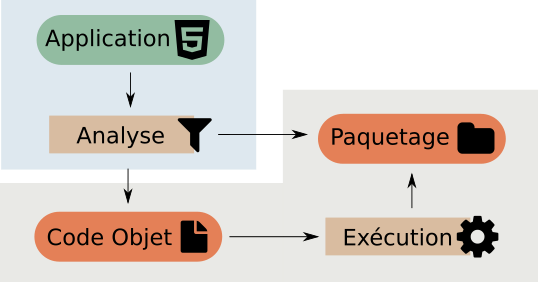
\includegraphics[scale=0.45]{execute} 
\caption{Schémas d'exécution}
\label{execute}
\end{figure}

\section{Perspectives}

De  ce premier  travail  il  en découle  un  ensemble de  perspectives
relatives à la compilation mais aussi à l'exécution.

\subsection{Compilation de document} 

Lors de  l'élaboration d'application l'injection de  code Thicket dans
toute page  HTML est pris  en charge dynamiquement. Cependant  lors du
passage au déploiement  une telle technique n'est pas  adaptée et peut
être couteuse.  La phase de  compilation existante dans un  client Web
peut être  alors reprise et intégrée  dans une phase de  compilation à
priori afin de  proposer une version optimale comme  cela est illustré
dans la figure \ref{precompile}.

\begin{figure}[h]
\centering
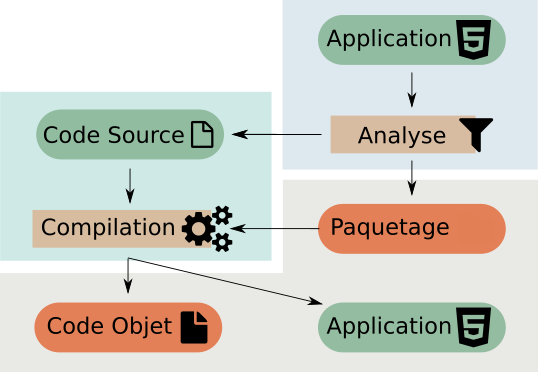
\includegraphics[scale=0.45]{precompile} 
\caption{Schémas de compilation de document HTML}
\label{precompile}
\end{figure}

Ce  type  de   technique  est  notamment  appliquée   par  des  outils
d'assemblage comme Bower \cite{bower} dans le monde du Web.

\subsection{Sécurisation du code objet}

Avec la maîtrise de cette problématique d'exécution et de distribution
l'aspect sécurité peut être entre autres revisité par la mise en place
de  système  de  signature  de  code objet  et  de  paquetage.   Cette
technique doit permettre de garantir l'intégrité du code objet.

\subsection{Paquetage et distribution}

Un  dernier aspect  concerne la  mise à  disposition de  paquetage. En
effet,  les  deux schémas  mettent  en  évidence  un mécanisme  lié  à
l'utilisation de tels paquetages.  Couplé avec la sécurisation du code
objet,  des solutions  basées sur  la  dissimination par  le biais  de
réseau de  diffusion de contenu  (CDN) peuvent être  envisagées.  Ceci
doit permettre  de mettre en place  une forme pervasive du  support du
langage que ce soit en terme  de module pour l'analyse, la compilation
et l'exécution  mais aussi en terme  de code objet disponibles  sur le
réseau.

\section{Conclusion}

Une  telle expérimentation  nous  permet d'explorer  non seulement  le
domaine des langages d'un point de  vue formel mais aussi, chose aussi
importante  son intégration  dans  des  écosystèmes distribués.   Cela
couvre  notamment la  capacité du  language à  supporter l'élaboration
d'applications  dites riches  ainsi que  la prise  en charge  en terme
d'exécution et de distribution à travers  le réseau par la gestion des
paquetages.

\bibliographystyle{abbrv}
\bibliography{mesreferences}

\end{document}


